\documentclass[9pt,parskip]{scrartcl}
%\documentclass[10pt,parskip]{scrartcl}
\usepackage{calc}
\usepackage{braket}
\usepackage[landscape,paper=a3paper,left=2mm, right=2mm,top=1.5mm, bottom = 3mm,includehead,headheight=3.5mm,headsep=1.5mm]{geometry}
\usepackage{multicol}
%Fr angepasste Aufzhlungen ohne Abstnde
\usepackage[alwaysadjust]{paralist}

%

%++++++++++++++++++++++++++++++++++++++ MEINE SACHEN
\usepackage[ngerman]{babel} % Unterstuetzung fuer deutsche Trennung und
%   zB Datum-Formatierung

%\usepackage{cmbright} % CMBRIGHT für alles! aus Formeln , weglassen für  Computer Modern und Roman Math 
\usepackage[utf8]{inputenc} % Einfache Eingabe von Umlauten

\usepackage[T1]{fontenc}
\renewcommand*\familydefault{\sfdefault}

\usepackage{multirow} % Zeilenzusammen nehmen
%\usepackage{lpic} % text über grafiken

%\renewcommand\familydefault{\rmdefault}
\usepackage[]{amsmath}   % diese zwei Pakete werden hier nicht
\usepackage{amssymb}   % gebraucht sind aber sehr sinnvoll
\usepackage{amsfonts}
\usepackage{empheq}
\usepackage{color}
\usepackage{graphicx}
\usepackage{subfigure}
\usepackage{float} % for [H]
\usepackage{arydshln}
\usepackage[]{algorithm2e}
\usepackage{bbm}
%\usepackage{xcolor}

%\usepackage[derived]{SIunits} %Units
\graphicspath{/}
%\usepackage{listings}  keine Ahung lol

 %PLATZSPAAREN SPACING 
\setlength{\parskip}{0pt}
\setlength{\parsep}{0pt}

%%%%%%%%%%%%%%%%%%%%%%%%%%%%%%%%%% bobs stuff %%%%%%%%%%%%%%%%%%%%%%%%%%%%%%%%%%%%%%%%%%%%%%%%%%%%%%%%%%%%%%%%%%%%%%%%%%%%%%%%%%%%%%%%%%%%%%%%%%%%%%%%%%%%%%%%%%%%%%%%%%%%%%%%
\usepackage{enumitem}
\setlist{nolistsep} 
%% code from mathabx.sty and mathabx.dcl
\DeclareFontFamily{U}{mathx}{\hyphenchar\font45}
\DeclareFontShape{U}{mathx}{m}{n}{
      <5> <6> <7> <8> <9> <10>
      <10.95> <12> <14.4> <17.28> <20.74> <24.88>
      mathx10
      }{}
\DeclareSymbolFont{mathx}{U}{mathx}{m}{n}
\DeclareFontSubstitution{U}{mathx}{m}{n}
\DeclareMathAccent{\widecheck}{0}{mathx}{"71}
\DeclareMathAccent{\wideparen}{0}{mathx}{"75}

\def\cs#1{\texttt{\char`\\#1}}

\usepackage{cancel}
\setlength{\arraycolsep}{2pt}
\setlength{\tabcolsep}{2pt}
\usepackage[dvipsnames]{xcolor}

\usepackage{pbox}
\usepackage{fancybox}

\newcommand*{\Scale}[2][4]{\scalebox{#1}{$#2$}}%
\newcommand*{\Resize}[2]{\resizebox{#1}{!}{$#2$}}%
\newcommand{\norm}[1]{\left\lVert#1\right\rVert}

%%%%%%%%%%%%%%%%%%%%%%%%%%%%%%%%%%%%%%%%%%%%%%%%%%%%%%%%%%%%%%%%%%%%%%%%%%%%%%%%%%%%%%%%%%%%%%%%%%%%%%%%%%%%%%%%%%%%%%%%%%%%%%%%%%%%%%%%%%%%%%%%%%%%%%%%%%%%%%%%%%%%%%%%%%%%%%%%

\usepackage[]{titlesec} % SPACING überall definieren
\titlespacing*{\section}{0pt}{0.15cm}{0.15cm} %indent,space befor, space after
\titlespacing*{\subsection}{0pt}{3pt}{3pt}
\titlespacing*{\subsubsection}{0pt}{0.15cm}{0pt}
\titleformat*{\section}{\fontencoding{OT1}\fontfamily{cmr} \fontseries{bx}\fontshape{sc} \fontsize{14pt}{14pt} \selectfont \color{Bittersweet}}%italic
\titleformat*{\subsection}{\fontencoding{OT1}\fontfamily{cmr} \fontseries{bx}\fontshape{sc} \fontsize{12pt}{12pt} \selectfont \color{YellowOrange}} %italic
\titleformat*{\subsubsection}{\fontencoding{OT1}\fontfamily{cmr} \fontseries{bx}\fontshape{sc} \fontsize{8pt}{8pt} \selectfont} %italic
\def\thesection{\arabic{subsection}}
\def\thesubsection{\arabic{subsection}}

%\setlength\headsep{9pt}
\setlength\columnseprule{0.5pt}

% Abstände vor und nach Grafiken verkleinern
\usepackage[belowskip=-15pt,aboveskip=0pt]{caption}
\setlength{\intextsep}{2pt plus 2pt minus 0pt}

%\setlength{\abovedisplayskip}{0pt}
%\setlength{\abovedisplayshortskip}{2pt}
%\setlength{\belowdisplayskip}{5pt}
%\setlength{\belowdisplayshortskip}{2pt}

%Macros reinladen
%% MACROS %%

\def\(({\left(}
\def \xyz{ \(( \begin{array}{ccc }
    x \\
  y \\
  z
\end{array}\))
}
\def \sphere{ \(( \begin{array}{ ccc}
    r \\
  \theta \\
  \phi
\end{array} \))
}
\def\)){\right)}
\newcommand{\diffn}[2]{\frac{d \ #1}{d  #2}}
\newcommand{\diffp}[2]{\frac{\partial  #1}{\partial   #2}}

\newcommand{\myv}[3]{ \(( \begin{array}{ccc}
    #1 \\
  #2 \\
  #3
\end{array}\))
}

\newcommand{\bild}[3]{
\begin{figure}[H]  
 \centering
    \includegraphics[#3]{#1}
    \caption{#2}
\end{figure}
}

\newcommand{\bildlabel}[4]{
\begin{figure}[h]  
 \centering
    \includegraphics[#3]{#1}
    \caption{#2}
    \label{#4}
\end{figure}
}

\newcommand{\bildo}[2]{
\begin{figure}[H]  
 \centering
    \includegraphics[#2]{#1}
\end{figure}
}

\newcommand{\un}{\underline}
%Fr fbox:
\newcommand{\f}{\fbox}


\newcommand{\ra}{\rightarrow}
\newcommand{\s}{\sigma}
\newcommand{\e}{\epsilon}

\newcommand{\al}[1]
{\begin{align*}
#1
\end{align*}
}

\newcommand{\aln}[1]
{\begin{align}
#1
\end{align}
}

%% Emphasize Math ==============================
\definecolor{insidecolor}{rgb}{0.93,0.93,0} 
\definecolor{border}{rgb}{0,0,0}
 
\newcommand*\mybluebox[1]{% 
\fcolorbox{border}{insidecolor}{\hspace{1em}#1\hspace{1em}}
}

\newcommand{\eal}[1]
{\begin{empheq}[box=\mybluebox]{align*} 
#1
\end{empheq}
}

\newcommand{\ealn}[1]
{\begin{empheq}[box=\mybluebox]{align} 
#1
\end{empheq}
}

\newcommand{\emult}[1]
{\begin{empheq}[box=\mybluebox]{multline*} 
#1
\end{empheq}
}
\newcommand{\emultn}[1]
{\begin{empheq}[box=\mybluebox]{multline} 
#1
\end{empheq}
}
%==========================================

\newcommand{\tsf}[1]
{\textsf{#1}
}

\newcommand{\tbf}[1]
{\textbf{#1}
}


\newcommand{\fal}[1]
{\begin{flalign*}
#1
\end{flalign*}
}

\newcommand{\ocirc}[1]{\buildrel _{\circ} \over {\mathbf{#1}}}

\newenvironment{fminipage}%
{\begin{Sbox}\begin{minipage}}%
{\end{minipage}\end{Sbox}\fbox{\TheSbox}}



\newenvironment{mybulletlist}
{%begin
\begin{list}{\RIGHTarrow}
{\setlength{\topsep}{0cm} 
\setlength{\parsep}{2mm}
\setlength{\leftmargin}{1.5cm}
\setlength{\rightmargin}{0cm}
\setlength{\labelwidth}{2cm} 
\setlength{\labelsep}{0.5cm}}
}
{%end
\end{list} 
}

\newcounter{linie}
\newenvironment{mynumberlist}
{%begin

\begin{list}{\thelinie .} 
{\usecounter{linie} 
\setlength{\topsep}{0cm} 
\setlength{\parsep}{4mm}
\setlength{\leftmargin}{2cm}
\setlength{\rightmargin}{1.5cm}
\setlength{\labelwidth}{2cm} 
\setlength{\labelsep}{0.5cm}} 
}
{%end
\end{list} 
}

\newenvironment{mybulletlistref}
{%begin
\begin{list}{$\mathbf{\dashrightarrow}$}
{\setlength{\topsep}{0cm} 
\setlength{\parsep}{4mm} 
\setlength{\leftmargin}{2cm}
\setlength{\rightmargin}{1.5cm}
\setlength{\labelwidth}{2cm} 
\setlength{\labelsep}{0.5cm}}
}
{%end
\end{list} 
}



%% MACROS %% end 

\newcommand{\dt}{\textnormal{d}t}
\newcommand{\deta}{\textnormal{d}\eta}
\newcommand{\argmin}{\mathop{\mathrm{argmin}}}
\newcommand{\Upr}{{\mathop{\mathrm{Upr}}}}
\newcommand{\Sgn}{{\mathop{\mathrm{Sgn}}}}
\newcommand{\h}{\mathop{\mathrm{H}}}
\newcommand{\prox}{{\mathop{\mathrm{prox}}}}
\newcommand{\abs}{\mathop{\mathrm{abs}}}
\newcommand{\T}{^{\mathop{\mathrm{T}}}}
\newcommand{\diag}{{\mathop{\mathrm{diag}}}}


%boldmath
%bold greek
\newcommand{\val}{\mbox{\boldmath $\alpha$}}
\newcommand{\vbe}{\mbox{\boldmath $\beta$}}
\newcommand{\vga}{\mbox{\boldmath $\gamma$}}
\newcommand{\vde}{\mbox{\boldmath $\delta$}}
\newcommand{\vep}{\mbox{\boldmath $\epsilon$}}
\newcommand{\vze}{\mbox{\boldmath $\zeta$}}
\newcommand{\vet}{\mbox{\boldmath $\eta$}}
\newcommand{\vth}{\mbox{\boldmath $\theta$}}
\newcommand{\vio}{\mbox{\boldmath $\iota$}}
\newcommand{\vka}{\mbox{\boldmath $\kappa$}}
\newcommand{\vla}{\mbox{\boldmath $\lambda$}}
\newcommand{\vmu}{\mbox{\boldmath $\mu$}}
\newcommand{\vnu}{\mbox{\boldmath $\nu$}}
\newcommand{\vxi}{\mbox{\boldmath $\xi$}}
\newcommand{\vpi}{\mbox{\boldmath $\pi$}}
\newcommand{\vrh}{\mbox{\boldmath $\rho$}}
\newcommand{\vsi}{\mbox{\boldmath $\sigma$}}
\newcommand{\vta}{\mbox{\boldmath $\tau$}}
\newcommand{\vup}{\mbox{\boldmath $\upsilon$}}
\newcommand{\vph}{\mbox{\boldmath $\varphi$}}
\newcommand{\vch}{\mbox{\boldmath $\chi$}}
\newcommand{\vps}{\mbox{\boldmath $\psi$}}
\newcommand{\vom}{\mbox{\boldmath $\omega$}}

\newcommand{\vvep}{\mbox{\boldmath $\varepsilon$}}
\newcommand{\vvth}{\mbox{\boldmath $\vartheta$}}
\newcommand{\vvrh}{\mbox{\boldmath $\varrho$}}
\newcommand{\vvpi}{\mbox{\boldmath $\varpi$}}
\newcommand{\vvsi}{\mbox{\boldmath $\varsigma$}}
\newcommand{\vvph}{\mbox{\boldmath $\phi$}}

%bold capital greek
\newcommand{\vGa}{\mathbf \Gamma}
\newcommand{\vDe}{\mathbf \Delta}
\newcommand{\vTh}{\mathbf \Theta}
\newcommand{\vLa}{\mathbf \Lambda}
\newcommand{\vXi}{\mathbf \Xi}
\newcommand{\vPi}{\mathbf \Pi}
\newcommand{\vSi}{\mathbf \Sigma}
\newcommand{\vUp}{\mathbf \Upsilon}
\newcommand{\vPh}{\mathbf \Phi}
\newcommand{\vPs}{\mathbf \Psi}
\newcommand{\vOm}{\mathbf \Omega}

%capital greek slanted, OHNE amsmath-package
%\newcommand{\iGa}{\mathnormal{\Gamma}}
%\newcommand{\iDe}{\mathnormal{\Delta}}
%\newcommand{\iTh}{\mathnormal{\Theta}}
%\newcommand{\iLa}{\mathnormal{\Lambda}}
%\newcommand{\iXi}{\mathnormal{\Xi}}
%\newcommand{\iPi}{\mathnormal{\Pi}}
%\newcommand{\iSi}{\mathnormal{\Sigma}}
%\newcommand{\iUp}{\mathnormal{\Upsilon}}
%\newcommand{\iPh}{\mathnormal{\Phi}}
%\newcommand{\iPs}{\mathnormal{\Psi}}
%\newcommand{\iOm}{\mathnormal{\Omega}}

%capital greek slanted, MIT amsmath-package
\newcommand{\iGa}{\varGamma}
\newcommand{\iDe}{\varDelta}
\newcommand{\iTh}{\varTheta}
\newcommand{\iLa}{\varLambda}
\newcommand{\iXi}{\varXi}
\newcommand{\iPi}{\varPi}
\newcommand{\iSi}{\varSigma}
\newcommand{\iUp}{\varUpsilon}
\newcommand{\iPh}{\varPhi}
\newcommand{\iPs}{\varPsi}
\newcommand{\iOm}{\varOmega}

%bold latin
\newcommand{\va}{\mathbf a}
\newcommand{\vb}{\mathbf b}
\newcommand{\vc}{\mathbf c}
\newcommand{\vd}{\mathbf d}
\newcommand{\ve}{\mathbf e}
\newcommand{\vf}{\mathbf f}
\newcommand{\vg}{\mathbf g}
\newcommand{\vh}{\mathbf h}
\newcommand{\vi}{\mathbf i}
\newcommand{\vj}{\mathbf j}
\newcommand{\vk}{\mathbf k}
\newcommand{\vl}{\mathbf l}
\newcommand{\vm}{\mathbf m}
\newcommand{\vn}{\mathbf n}
\newcommand{\vo}{\mathbf o}
\newcommand{\vp}{\mathbf p}
\newcommand{\vq}{\mathbf q}
\newcommand{\vr}{\mathbf r}
\newcommand{\vs}{\mathbf s}
\newcommand{\vt}{\mathbf t}
\newcommand{\vu}{\mathbf u}
\newcommand{\vv}{\mathbf v}
\newcommand{\vw}{\mathbf w}
\newcommand{\vx}{\mathbf x}
\newcommand{\vy}{\mathbf y}
\newcommand{\vz}{\mathbf z}
\newcommand{\eins}{\mathbf 1}

%bold capital latin
\newcommand{\vA}{\mathbf A}
\newcommand{\vB}{\mathbf B}
\newcommand{\vC}{\mathbf C}
\newcommand{\vD}{\mathbf D}
\newcommand{\vE}{\mathbf E}
\newcommand{\vF}{\mathbf F}
\newcommand{\vG}{\mathbf G}
\newcommand{\vH}{\mathbf H}
\newcommand{\vI}{\mathbf I}
\newcommand{\vJ}{\mathbf J}
\newcommand{\vK}{\mathbf K}
\newcommand{\vL}{\mathbf L}
\newcommand{\vM}{\mathbf M}
\newcommand{\vN}{\mathbf N}
\newcommand{\vO}{\mathbf O}
\newcommand{\vP}{\mathbf P}
\newcommand{\vQ}{\mathbf Q}
\newcommand{\vR}{\mathbf R}
\newcommand{\vS}{\mathbf S}
\newcommand{\vT}{\mathbf T}
\newcommand{\vU}{\mathbf U}
\newcommand{\vV}{\mathbf V}
\newcommand{\vW}{\mathbf W}
\newcommand{\vX}{\mathbf X}
\newcommand{\vY}{\mathbf Y}
\newcommand{\vZ}{\mathbf Z}

%calligraphic
\newcommand{\cA}{\mathcal{A}}
\newcommand{\cB}{\mathcal{B}}
\newcommand{\cC}{\mathcal{C}}
\newcommand{\cD}{\mathcal{D}}
\newcommand{\cE}{\mathcal{E}}
\newcommand{\cF}{\mathcal{F}}
\newcommand{\cG}{\mathcal{G}}
\newcommand{\cH}{\mathcal{H}}
\newcommand{\cI}{\mathcal{I}}
\newcommand{\cJ}{\mathcal{J}}
\newcommand{\cK}{\mathcal{K}}
\newcommand{\cL}{\mathcal{L}}
\newcommand{\cM}{\mathcal{M}}
\newcommand{\cN}{\mathcal{N}}
\newcommand{\cO}{\mathcal{O}}
\newcommand{\cP}{\mathcal{P}}
\newcommand{\cQ}{\mathcal{Q}}
\newcommand{\cR}{\mathcal{R}}
\newcommand{\cS}{\mathcal{S}}
\newcommand{\cT}{\mathcal{T}}
\newcommand{\cU}{\mathcal{U}}
\newcommand{\cV}{\mathcal{V}}
\newcommand{\cW}{\mathcal{W}}
\newcommand{\cX}{\mathcal{X}}
\newcommand{\cY}{\mathcal{Y}}
\newcommand{\cZ}{\mathcal{Z}}

%fraktur
\newcommand{\frA}{\mathfrak{A}}
\newcommand{\frB}{\mathfrak{B}}
\newcommand{\frC}{\mathfrak{C}}
\newcommand{\frD}{\mathfrak{D}}
\newcommand{\frE}{\mathfrak{E}}
\newcommand{\frF}{\mathfrak{F}}
\newcommand{\frG}{\mathfrak{G}}
\newcommand{\frH}{\mathfrak{H}}
\newcommand{\frI}{\mathfrak{I}}
\newcommand{\frJ}{\mathfrak{J}}
\newcommand{\frK}{\mathfrak{K}}
\newcommand{\frL}{\mathfrak{L}}
\newcommand{\frM}{\mathfrak{M}}
\newcommand{\frN}{\mathfrak{N}}
\newcommand{\frO}{\mathfrak{O}}
\newcommand{\frP}{\mathfrak{P}}
\newcommand{\frQ}{\mathfrak{Q}}
\newcommand{\frR}{\mathfrak{R}}
\newcommand{\frS}{\mathfrak{S}}
\newcommand{\frT}{\mathfrak{T}}
\newcommand{\frU}{\mathfrak{U}}
\newcommand{\frV}{\mathfrak{V}}
\newcommand{\frW}{\mathfrak{W}}
\newcommand{\frX}{\mathfrak{X}}
\newcommand{\frY}{\mathfrak{Y}}
\newcommand{\frZ}{\mathfrak{Z}}

\newcommand{\fra}{\mathfrak{a}}
\newcommand{\frb}{\mathfrak{b}}
\newcommand{\frc}{\mathfrak{c}}
\newcommand{\frd}{\mathfrak{d}}
\newcommand{\fre}{\mathfrak{e}}
\newcommand{\frf}{\mathfrak{f}}
\newcommand{\frg}{\mathfrak{g}}
\newcommand{\frh}{\mathfrak{h}}
\newcommand{\fri}{\mathfrak{i}}
\newcommand{\frj}{\mathfrak{j}}
\newcommand{\frk}{\mathfrak{k}}
\newcommand{\frl}{\mathfrak{l}}
\newcommand{\frm}{\mathfrak{m}}
\newcommand{\frn}{\mathfrak{n}}
\newcommand{\fro}{\mathfrak{o}}
\newcommand{\frp}{\mathfrak{p}}
\renewcommand{\frq}{\mathfrak{q}}
\newcommand{\frr}{\mathfrak{r}}
\newcommand{\frs}{\mathfrak{s}}
\newcommand{\frt}{\mathfrak{t}}
\newcommand{\fru}{\mathfrak{u}}
\newcommand{\frv}{\mathfrak{v}}
\newcommand{\frw}{\mathfrak{w}}
\newcommand{\frx}{\mathfrak{x}}
\newcommand{\fry}{\mathfrak{y}}
\newcommand{\frz}{\mathfrak{z}}



%%Header
\usepackage{fancyhdr}
\pagestyle{fancy}
\rhead{Christoph Zuidema 13-913-314 czuidema@student.ethz.ch}
\lhead{Page \thepage}
\chead{Statistical Learning Theory - Summary}

%++++++++++++++++++++++++++++++++++++++++++++++++++++++++++++++++++++++++
\newcommand{\E}{\textrm{E}}
\newcommand{\V}{\textrm{Var}}

\makeatletter
\g@addto@macro\normalsize{%
  \setlength\abovedisplayskip{0pt}
  \setlength\belowdisplayskip{0pt}
  \setlength\abovedisplayshortskip{0pt}
  \setlength\belowdisplayshortskip{0pt}
}
\makeatother

\begin{document}
\begin{multicols*}{4}


\section*{Basics}
\subsection*{General}
\textit{Cauchy-Schwartz Inequality: }$|u\cdot v|\le \|u\|\|v\|$ \\
\textit{Gauss distribution:}\\
$f_{\mathbf{X} }(x_{1},\ldots ,x_{k})=\frac {\exp \left(-{\frac {1}{2}}({\mathbf {x} }-{\boldsymbol {\mu }})^{\mathrm {T} }{\boldsymbol {\Sigma }}^{-1}({\mathbf {x} }-{ \boldsymbol {\mu }})\right)}{\sqrt {(2\pi )^{k}|{\boldsymbol {\Sigma }}|}}$ 
\subsection*{Probability Basics}
$\Pr[a\leq X\leq b]=\int _{a}^{b}f_{X}(x)\,dx$ \\
\textit{Cumulative distribution function: } $F_{X}(x)=\operatorname {P} (X\leq x) =\int _{-\infty }^{x}f_{X}(t)\,dt$ \\
\textit{Bayes: } $p(\theta |x)={\frac {p(x|\theta )p(\theta )}{p(x)}} = p(\text{model} | \text{data} )={\frac {p( \text{data}|\text{model} )p(\text{model})}{p(\text{data})}} $ \\
$\text{Posterior probability} \propto \text{Likelihood} \times \text{Prior probability}$ \\
\textit{Markov inequality} $\mathbb{P}(g(X) \geq r) \leq \dfrac{\mathbb{E}[g(X)]}{r}$ \\
\textit{Chebyshev inequality} $\mathbb{P}(|X-\mu|\geq \epsilon) \leq \frac{\sigma^2}{\epsilon^2}$ \\
\textit{Jensen inequality} $\varphi \left(\operatorname {E} [X]\right)\leq \operatorname {E} \left[\varphi (X)\right]$ where $\varphi$ is a \textit{convex} function. E.g. $log(x)$ if $x > 0$ \\
\textit{Law of large numbers} $\mathbb{P}(|\frac{S_n}{n}-\mu|\geq \epsilon) \leq \frac{\sigma^2}{n \cdot \epsilon^2} \to 0$ if $n \to 0$ \\
\textit{Bound on disjunction: }$\max{\mathbb{P}(A_1), \dots , \mathbb{P}(A_n)} \leq \mathbb{P}(E) \leq \min{1, \mathbb{P}(A_1) + \dots + \mathbb{P}(A_n)}$

\textit{Glivenko-Catelli theorem: }$\mathbb{P}(\sup_{x} | F_{n}(x) - F(x)| \to 0)=1$ if $n \to 0$.

\textit{Completing the square: }
If we want to go from $ax^2 + bx + c = 0$ to $a(x+d)^2 + e = 0$, 
we get $d$ by $d = \frac{b}{2a}$ and $e = c - \frac{b^2}{4a}$
\subsection*{Derivatives}
$\frac{\partial}{\partial \mathbf{x}}(\mathbf{b}^\top \mathbf{x}) = \frac{\partial}{\partial \mathbf{x}}(\mathbf{x}^\top \mathbf{b}) = \mathbf{b}$ \quad
$\frac{\partial}{\partial \mathbf{x}}(\mathbf{x}^\top \mathbf{x}) = 2\mathbf{x}$\\
$\frac{\partial}{\partial \mathbf{x}}(\mathbf{x}^\top \mathbf{A}\mathbf{x}) = (\mathbf{A}^\top + \mathbf{A})\mathbf{x}$ \quad
$\frac{\partial}{\partial \mathbf{x}}(\mathbf{b}^\top \mathbf{A}\mathbf{x}) = \mathbf{A}^\top \mathbf{b}$\\
$\frac{\partial}{\partial \mathbf{X}}(\mathbf{c}^\top \mathbf{X} \mathbf{b}) = \mathbf{c}\mathbf{b}^\top$ \quad
$\frac{\partial}{\partial \mathbf{X}}(\mathbf{c}^\top \mathbf{X}^\top \mathbf{b}) = \mathbf{b}\mathbf{c}^\top$\\
$\frac{\partial}{\partial \mathbf{x}}(\| \mathbf{x}-\mathbf{b} \|_2) = \frac{\mathbf{x}-\mathbf{b}}{\|\mathbf{x}-\mathbf{b}\|_2}$ \quad
$\frac{\partial}{\partial \mathbf{x}}(\|\mathbf{x}\|^2_2) = \frac{\partial}{\partial \mathbf{x}} (\mathbf{x}^\top \mathbf{x}) = 2\mathbf{x}$\\
$\frac{\partial}{\partial \mathbf{X}}(\|\mathbf{X}\|_F^2) = 2\mathbf{X}$ \quad
$\frac{\partial}{\partial \mathbf{X}}(\|\mathbf{X}\|_2) = \frac{x}{\|\mathbf{X}\|_2}$ \\ 

$\frac{\partial}{\partial \mathbf{x}}(\|\mathbf{Ax - b}\|_2^2) = \mathbf{2(A^\top Ax-A^\top b)}$
$\frac{\partial}{\partial x}\frac{g(x)}{h(x)} = \frac{g'(x)h(x) - g(x)h'(x)}{h(x)^2}$\\
$\frac{\partial}{\partial(w_i^Tx)}softmax(j)= softmax(j)(\delta_{ij} - softmax(i))$

For functionals, we have the Taylor approximation of: $F[x + \epsilon \eta] = F[X] + \epsilon \int \frac{\partial F}{\partial x}(z) \eta (z) dz + O(\epsilon ^2)$

\subsection*{Maximization Basics}
\subsubsection*{Calculus of Variations}
Goal: find the maximum of a functional. \\
$J(x + \delta x) - J(x) = 0$ \\
Given: functional of form 
$J[f]=\int _{a}^{b} L[x,f(x),f'(x)] dx $ \\
change $\delta J = \int_a^b  \frac{\delta J}{\delta f(x)} \delta f(x) dx $ \\
\textit{complete data likelihood:} $p(x,k|\mu, \eta)$\\
\textit{incomplete data likelihood:} $p(x|\mu, \eta)$\\
functional derivative (Euler Lagrange): $\frac{\delta J}{\delta f(x)} = \frac{\partial L}{\partial f} -\frac{d}{dx} \frac{\partial L}{\partial f'} $
\subsubsection*{EM-Algorithm}
\textit{given}: $p(\mathbf{X},\mathbf{Z}|\mathbf{\theta})$ with observed variables $\mathbf{X}$ and latent variables $\mathbf{Z}$, parameters $\mathbf{\theta}$
\textit{goal:} maximize likelihood function $p(\mathbf{X}|\mathbf{\theta})$ wrt. $\mathbf{\theta}$.
\begin{enumerate}
	\item choose initial setting for $\boldsymbol{\theta}^{old}$
	\item \textbf{E-step:} evaluate 
	$Q_i(z^{(i)}) := p(z^{(i)}|x^{(i)};\theta)$
	\item \textbf{M-step:} 
	$\theta := argmax_{\theta} \sum_i \sum_{z^{(i)}} Q_i(z^{(i)})log\frac{p(x^{(i)},z^{(i)};\theta)}{Q_i(z^{(i)})}$ 
	\item check if converged.
\end{enumerate}

\subsection*{Information Theory}
\textit{Mutual information: } \\
measures the amount of information that can be obtained about one random variable by observing another \\
$I(X;Y)=\mathbb {E} _{X,Y}[SI(x,y)]=\sum _{x,y}p(x,y)\log {\frac {p(x,y)}{p(x)\,p(y)}}$ \\
$I(X;Y)=H(X)-H(X|Y).\,$ \\
$I(X;Y)=I(Y;X)=H(X)+H(Y)-H(X,Y).\,$ \\
$I(X,Y;Z) = I(X;Z) + I(Y;Z|X)$\\
\textit{chain rule for information: }$I(X;Y,Z)=I(X;Z)+I(X;Y|Z)$ \\
$I(X;Y)=\mathbb {E} _{p(y)}[D_{\mathrm {KL} }(p(X|Y=y)\|p(X))].$ \\
\textit{Information Processing Inequality: } Let $X \rightarrow Y \rightarrow Z$ be a Markov Chain, then $I(x,z) \leq I(x,y)$
\subsection*{Kullback-Leibler divergence}
\begin{itemize}
	\item quantifies coding cost describing data with probability distribution $q$ when true distribution is $p$.
	\item KL divergence is positive semidefinite. $D_{\mathrm {KL} } \geq 0$. Use Jensen's inequality to prove it. 
\end{itemize}
way of comparing two distributions: a "true" probability distribution $p(X)$, and an arbitrary probability distribution $q(X)$. \\
or: "unnecessary surprise". \textbf{not} symmetric! \\
q(X) is the distribution underlying some data, when, in reality, p(X) is the correct distribution, the Kullback–Leibler divergence is the number of average additional bits per datum necessary for compression. \\
$D_{\mathrm {KL} }(p(X)\|q(X))=\sum _{x\in X}-p(x)\log {q(x)}\,-\,\sum _{x\in X}-p(x)\log {p(x)}=\sum _{x\in X}p(x)\log {\frac {p(x)}{q(x)}}$ \\
continuous case: $D_{\mathrm {KL} }(P\|Q)=\int _{-\infty }^{\infty }p(x) \log {\frac {p(x)}{q(x)}} dx$ \\



\section*{Dimensionality Reduction}
\subsection*{Principal Component Analysis (PCA)}
\subsubsection*{Idea}
dimensionality reduction with orthogonal projection of D-dimensional data onto lower M-dimensional linear space (\textit{principal subspace}). Variance is maximized.
\subsubsection*{Procedure}
\begin{enumerate}
	\item calculate mean $\bar{x} = \frac 1 N \sum_{n=1}^{N}x_n$ and covariance matrix \textbf{S} of data set
	\item find the $M$ eigenvectors corresponding to the $M$ largest eigenvalues.
	\item data projected on these eigenvectors have largest variance.
\end{enumerate}
\subsection*{Probabilistic Principal Component Analysis (PPCA)}
\subsubsection*{Idea}
$\mathbf{x} = \mathbf{Wz} + \boldsymbol{\mu} + \boldsymbol{\epsilon} $, with $p(\mathbf{z}) = \mathcal{N}(\mathbf{z}|\mathbf{0,I})$ and $\epsilon ~ \mathcal{N}(0, \sigma^2\mathbf{I})$ \\
$p(\mathbf{x}|\mathbf{z}) = \mathcal{N}(\mathbf{x}|\mathbf{Wz} + \boldsymbol{\mu}, \sigma^2\mathbf{I}) $
\subsubsection*{Procedure}
\begin{enumerate}
	\item calculate mean $\bar{x} = \frac 1 N \sum_{n=1}^{N}x_n$ and covariance matrix \textbf{S} of data set
	\item find the $M$ eigenvectors corresponding to the $M$ largest eigenvalues.
	\item data projected on these eigenvectors have largest variance.
\end{enumerate}
\subsubsection*{Advantages}
\begin{itemize}
	\item computationally efficient $\to$ no need to evaluate covariance matrix as intermediate step
	\item allows us to deal with missing data in data set
\end{itemize}


\subsection*{Locally Linear Embedding}
$N$ real valued vector $\vec{X}_i $ of dimension $D$.\\
\textit{Assumption: } data lies close on locally linear patch of manifold. \\
Construct each data point form its $K$ nearest (e.g. euclidean distance) neighbors. \\
\textit{Reconstruction error: }$\mathcal{E} (W) = \sum_i |\vec{X}_i -  \sum_j W_{ij} \vec{X}_j|$ \\
where $W_{ij}$ summarize the contribution of the $j$th data point to
the $i$th reconstruction. \\
\underline{\textit{LLE Algorithm: }} \\
\shadowbox{
\parbox{0.95\linewidth}{
\begin{minipage}{0.75\linewidth}
\begin{enumerate}
\item Compute the neighbors of each data point, $\vec{X}_i $.
\item Compute the weights $W_{ij}$ that best reconstruct each data point $\vec{X}_i$ from its neighbors, minimizing the cost $\mathcal{E} (W) $ by constrained linear fits. We have $w_{ij} = \frac{\sum_k C_{jk}^{(-i)}}{\sum_{lk}C_{lk}^{(-i)}}$, where $C_{jk}^{(i)} = (x_i - x_j)^T(x_i - x_k)$
\item Compute the vectors $\vec{Y}_i$ best reconstructed by the weights $W_{ij}$, minimizing the quadratic form in $\Phi(Y) = \sum_i |\vec{X}_i -  \sum_j W_{ij} \vec{Y}_j|^2$ by its bottom nonzero eigenvectors.
The embedding vectors are given by the eigenvectors corresponding to the d+1 smallest eigenvalues of $M = (1 - W)^T(1-W)$

\end{enumerate}
\end{minipage}
}
}
\section*{Maximum Entropy Inference}
\textit{Maximizing entropy yields least biased inference method $\to$ maximally noncommittal wrt. missing data. }
\subsection*{Maximum entropy distribution}
\subsubsection*{Idea}
Outcomes $\omega_i \in \Omega$, determine probabilities $p_i = \mathbb{P}(\omega_i)$.
Given constraints/moments $\mu_i = \mathbb{E}[r_j] = \sum_{i=1}^n r_j(\omega_i)p_i$, where $r_j : \Omega \to \mathbb{R} j = 1, 2, ..., n$ are different functions defined over $\Omega$. 
\subsubsection*{Gibbs distribution}
\textit{minimal sesitivity to changes in constraint moments $\mu_i$} \\
$p(x) = \frac 1 Z \text{exp}(- \sum_{j=1}^m \lambda_j r_j(x))$ where $m$ is the number of constraints. \\

$Z = \int_x \text{exp}(- \sum_{j=1}^m \lambda_j r_j(x)) dx$
\subsubsection*{Gibbs Free Energy}
$G(p) = \sum_x p(x) E(x) + \frac{1}{\beta} \sum_x p(x)log p(x) = \frac{1}{\beta} D_{KL}(p||p_{\beta}) + F(\beta)$
Minimising $G(p)$ minimises the expected cost and maximises the entropy of $p(x)$.
\subsubsection*{Derive least sensitive distributions}
\begin{enumerate}
	\item determine all $r_j$ from constraints.
	\item calculate $Z$ and $p(x)$ from Gibbs distribution
	\item calculate all moments and set equal to constraints.
\end{enumerate}

For a general cost function:
\[\mathbf{P}(\mathbf{c}) = \frac{e^{-\beta \mathcal{R}(c)}}{\sum_{c' \in \mathcal{C} e^{-\beta \mathcal{R}(c')}}} = \frac{e^{-\beta \mathcal{R}(c)}}{Z} = \text{exp}(- \beta (\mathcal{R}(c)- \mathcal{F})) \]
where $\mathcal{F}(\beta) = -\frac 1 \beta \text{log}(Z)$ is known as "`free energy"'. \\
Free energy for any distribution: $\mathcal{F} = - \frac 1 \beta S(\mathbf{P}) + \mathbb{E}_{\mathbf{P}} \mathcal{R} $
\subsection*{Entropy}
$H_X$ of a discrete random variable $X$ is a measure of the amount of \textit{uncertainty} associated with the value of $X$ when only its distribution is known \\
$H(X)=\mathbb {E} _{X}[I(x)]=-\sum _{x\in \mathbb {X} }p(x)\log p(x)$ \\
$H(Y|X) = \sum_{x,y} p(x,y)log(p(y|x)$\\
\textit{Chain rule: } $ H(X,Y) = H(X) + H(Y|X) $ \\

$H(X,Y|Z) = H(X|Z) + H(Y|X,Z)$

\subsection*{Maximum Entropy Clustering}
\subsubsection*{Idea}
Determine probabilistic centroids $y_{\alpha}$ and probabilistic assignments $P_{i \alpha}$ of $i$-th object to cluster $\alpha$. Data $\mathcal{X}$ and labelings $c$ are r.v.

\subsubsection*{Procedure}
\begin{enumerate}
	\item Define posterior probability distribution $P(c|\mathcal{X},\mathcal{Y})$, $c \in \mathcal{C}$, constraint $\mathbb{E}_{P(c|\mathcal{X},\mathcal{Y})} \mathcal{R}(c,\mathcal{X},\mathcal{Y}) = \mu$ where $\mu$ is a constant.
	\item find centroid conditions and assignments $P_{i \alpha}$ by maximizing entropy wrt. $\mathcal{Y}$ $\to$ $\frac{\partial }{\partial \mathbf{y}_{\alpha}} H(P(c|\mathcal{X},\mathcal{Y})) = \mathbf{0}$
\end{enumerate}
Most agnostic $P(c|\mathcal{X},\mathcal{Y})$ is Gibbs distribution.  \\

\[P(c|\mathcal{X},\mathcal{Y})=\frac{\text{exp}(-\mathcal{R}(c,\mathcal{X},\mathcal{Y})/T)}{\sum_{c' \in \mathcal{C}} \text{exp}(-\mathcal{R}(c',\mathcal{X},\mathcal{Y})/T)}\]
\textit{Remark:} If the cost function is linear in individual costs, posterior can be factorized!

\subsection*{Clustering distributional data}
\subsubsection*{Idea}
"`Close"' objects have similar feature distributions. $\to$ cluster via similarity. \\
Distributional data encoded in dyads (pair $(x_i, y_i) \in \mathcal{X} \times \mathcal{Y} $): $n$ different objects $\{x_i\} \in \mathcal{X}$, $m$ possible feature values $\{y_i\} \in \mathcal{Y}$. Data is set of $l$ observations $\mathcal{Z} = \{ (x_{i(r)}, y_{j(r)})\}_{r=1}^{l}$. \\
Likelihood of data $\mathcal{Z}$ $\mathcal{L}(\mathcal{Z}) = \Pi_{i \leq n} \Pi_{j \leq m} P((i,j)|c(i),Q)^{l\hat{P}(i)}$ \\
where $l\hat{P}(i) =$ \# object $i$ exhibits value $j$ and $\hat{P}(i) $ = empirical probability finding object $i$ with feature value $j$.

\subsubsection*{Procedure}
\begin{enumerate}
	\item 
\end{enumerate}

\subsection*{Parametric distributional clustering}
Density estimation is assumed to be Gaussian $g_a(y)$. \\
$p(y| \nu) = \sum_{a \leq s} g_a(y) p(a|\nu)$ where $p(a|\nu)$ mixture coefficients, $s$ number of mixture components.\\
\textit{Remark:} Often feature values are restricted to specific domains, mixture components $\to$ rectified.
Complete data likelihood is given by: $p(x,M|\theta) = \prod_{i=1}^n \sum_{r=1}^k M_{ir}p_rp(x_i|r)$, where $M_{ir} \in \{0,1\}$ and $\sum_r M_{ir} = 1$

Assuming that the observations $x_{ij}$ are taken from domain $I$, which is equipartitioned into $I_p$ for $p= 1..m$, we have $p(x_{ij} \in i_p|\alpha) =: G_{\alpha}(p)$.
Thus:
$p(x,M|\theta) = \prod_{i=1}^n \prod_{r=1}^k[p_r \prod_{p=1}^m {\sum_{\alpha = 1}^l p(\alpha | r)G_{\alpha }(p)}^{n_{ip}}]^{M_{ir}}$,
where $n_{ip}$ counts how many observations $x_{ij}$ from object $i$ fell into bin $I_p$

The connection to the Info Bottleneck idea is given by:\\
$X$: decision to pick an object $i$ uniformly.\\
$\hat X$: encoding of object i by cluster r. \\
Y: Relative frequency of observing bin p.

Seeing that $I(X,\hat X) = H(X\hat X)$ = $-\sum_{r=1} p_r log p_r$, i.e. $I(X,\hat X) = log k$ for $p_r = \frac{1}{k}$

We also have $H(Y|\hat X) = - \sum_{i=1}^n \sum_{r=1}^k \sum_{p=1}^m M_{ir} \frac{n_{ip}}{n_i}\frac{1}{n} log \sum_{\alpha} p(\alpha|r)G_{\alpha}(p)$

Putting it all together we get that $I(X,\hat X) - \lambda I(\hat X, Y) = - \sum_r (\frac{1}{n}\sum_i M_{ir}) log p_r - \lambda \sum_{i,r} \frac{1}{n} M_{ir} \sum_p \frac{n_{ip}}{n_i}log \sum_{\alpha} p(\alpha|r)G_{\alpha}(p) - \lambda H(Y)
= - \frac{1}{n} \sum_{i,r} M_{ir}[log p_r + \frac{\lambda}{n_i} \sum_p n_{ip} log \sum_{\alpha} p(\alpha|r)G_{\alpha}(p)] - \lambda H(Y)$

By choosing the right constants and then dropping stuff that doesn't affect the minimum. That this is equal to the negative log likelihood. 

\subsection*{Markov Chain Monte Carlo (MCMC)}
\textit{Idea:} sampling from a probability distribution by constructing a Markov chain that has the desired distribution as its equilibrium distribution. 

\subsubsection*{Markov Chain}

$P_N (x_1,... ,x_N ) = p_1(x1) \prod^{N-1}_{t=1} w(x_t \to x_{t+1})$ \\ 
where $\{p_1(x)\}_{x \in \mathcal{X}}$ is the initial state and $\{w(x \to y)\}_{x,y \in \mathcal{X}}$ are the
transition probabilities \\
 transition probabilities must be
non-negative and normalized:
$\sum_{y \ in \mathcal{X}} w(x \to y) = 1 , \text{for any } y \in \mathcal{X}$
\textit{Eigenvalues: }\\
First eigenvalue is always equal to 1. The smaller $\lambda_2$ the faster the MCMC converges. \\
\textit{irreducible: } It is possible to get to any state from any state \\
\textit{Detailed balance: } $\pi _{i}P_{ij}=\pi _{j}P_{ji}$ or $p(x) (x \to y) = p(y) p(y \to x)$, implies stationarity! \\
\textit{Stationarity: } $\pi \mathbf {P} =\pi$ \\
\textit{Aperiodic: } Chain should not get trapped in cycles, i.e. for all states x,y there's an integer $n(x,y)$, s.t. $\forall n > n(x,y)$, there's a path of lenght $n$ between $x$ and $y$ \\


\subsubsection*{Metropolis-Hastings}
Initialization: Choose an arbitrary point $x_0$ as first sample, choose arbitrary probability density $g(x|y)$ that suggests a candidate for the next sample value x. For Metropolis algorithm, g must be symmetric $\to g(x|y)=g(y|x)$ e.g. a Gaussian distribution centered at y, $\to$ points closer to y more likely to be visited next $\to$ sequence of samples $\to$ random walk. function g $\to$ proposal density or jumping distribution. \\
\underline{\textit{Algorithm: }} \\
\shadowbox{
\parbox{0.95\linewidth}{
\begin{minipage}{0.75\linewidth}
\begin{enumerate}
\item Generate a new sample $x'$ from the old $x$ according to a proposal PDF: $x' \sim q(\, \mid x)$
\item Calculate acceptance probability $A(x',x)$ according to quotient $ Q(x',x) = \frac{p(x')q(x|x')}{p(x)q(x'|x)} $  $A(x' ,x) = min(1,Q(x',x))$
\item Accept $x'$ as new sample with with probability $A(x',x)$, else keep $x$.
\end{enumerate}
\end{minipage}
}
}
\textit{Disadvantages:}
\begin{itemize}
	\item samples are correlated. For independent samples one would have to take only every \textit{n}-th sample.
	\item initial samples may follow a very different distribution. Solution: throw away first 1000 samples.
	\item  for high dimensions: finding the right jumping distribution can be difficult, as the different individual dimensions behave in very different ways, and the jumping width must be "just right" for all dimensions at once to avoid excessively slow mixing $\to$ Gibbs Sampling.
\end{itemize}

\subsubsection*{Gibbs Sampling}
given a multivariate distribution it is simpler to sample from a conditional distribution than to marginalize by integrating over a joint distribution. \\
Applicable if:
\begin{itemize}
	\item conditional distribution of each variable is known and is easy (or at least, easier than joint distribution) to sample from
	\item 
\end{itemize}
For Gibbs sampling in the Ising model we use the transition probability to a new state where only $\sigma_i$ is flipped: $p_i(\sigma) = exp(-\beta max[0,\Delta E_i(\sigma)])$ 
 simulated annealing is often used to reduce the "random walk" behavior in the early part of the sampling process

\subsubsection*{Heat-Bath Algorithm}
Same as metropolis but with acceptance probability:
$$p(\sigma_{new}) = exp(-\beta E(\sigma_{new})) / ( exp(-\beta E(\sigma_{new}) + exp(-\beta E(\sigma_{old})))$$

\subsubsection*{Simulated Annealing}
\subsubsection*{Idea}
\begin{itemize}
	\item Markov process samples solution from solution space $\Omega$
	\item cost function $\mathcal{H}: \Omega \to \mathbb{R}, \omega \in \Omega$ denotes admissible solution.
	\item solutions accepted/rejected according to Metropolis algorithm: decreased cost $\to$ accepted, increased cost $\to$ accepted with probability $exp(- \Delta \mathcal{H}/T)$ where $\Delta \mathcal{H} = \mathcal{H}(\omega_{new}) - \mathcal{H}(\omega_{old}) $. $T$ is the computational temperature.
	\item reduce gradually the temperature during search proces $\to$ force system into solution with low costs. $\to$ random walk in solution space.
	\item annealing schedule, i.e. the $\beta$s, could be linear, quadratic of logarithmic for instance.

\end{itemize}
Markov process with converges to equilibrium: \\
$\mathbf{P^{Gb}(\omega)} = \text{exp}(-(\mathcal{H}(\omega) - \mathcal{F}(\mathcal{H}))/T )$ \\
where $\mathcal{F}(\mathcal{H})) = -T log \sum_{\omega' \in \Omega} \text{exp}(-\mathcal{H}(\omega')/T )$
\subsubsection*{Remarks}
\begin{itemize}
	\item Temperature formally $\approx$ Lagrange parameter $\to$ constraint on expected costs. $\braket{H} = \sum_{\omega \in \Omega} P^{Gb}(\omega)  \mathcal{H}(\omega)$
	\item Gibbs free energy related to expected cost via entropy $\mathcal{S}(P^{Gb}) = -\sum_{\omega \in \Omega} P^{Gb}(\omega)  \text{log} (P^{Gb}(\omega) ) = \frac 1 T \braket{H} - \frac 1 T \mathcal{F}(\mathcal{H})$
\end{itemize}

\subsubsection*{Parallel Tempering}
Two Monte Carlo simulation were to run in parallel, one at high and one at a low temperature. At certain steps we swap the configurations of the two runs. This way both runs have access to low and high temperature configuration improving convergence to a global optimum. We swap the configurations after each epoch.
\subsection*{Deterministic Annealing}
\subsubsection*{Idea}
deterministic variant of \textit{Simulated annealing}.

The critical temperature, at which a cluster will split is:
$T_c = 2\lambda_{max}$ where $\lambda_{max}$ is the largest eigenvalue of $C_{x|y_0} = \sum_x p(x|y)(x-y)(x-y)^t$

\subsection*{Information Bottleneck Method}
\subsubsection*{Idea}
input signal $X$ should be efficiently encoded by e.g. cluster variable $\tilde{X}$ preserving relevant information about context variable $Y$ as good as possible.

$ I(X; \tilde{X}) - \lambda I(\tilde{X}, Y)$

\subsection*{Parametric Distributional Clustering}
\subsubsection*{Idea}
cluster set of $n$ objects $\mathbf{o}_i$ in $k$ groups. Assignments encoded in $M_{i, \nu}$, $M_{i, \nu} = 1$ if $\mathbf{o}_i$ assigned to cluster $\nu$. Enforce $\sum_{\nu \leq k} M_{i, \nu} = 1$.

\section*{Graph based clustering}
\textit{relations among objects not necessarily metric.}
\subsubsection*{Idea}
$\mathcal{O}$ is the set of vertices $\mathcal{V}$, set of edges is inferred, set of (di)similarity measures $\mathcal{D}=\{D_{ij}\}$ or $\mathcal{S}=\{S_{ij}\}$ are the weights. \\
Cluster defined as: $\mathcal{G}_{\alpha} \{ \mathbf{o} \in \mathcal{O} : c( \mathbf{O}) = \alpha\}$
\subsection*{Correlation Clustering}
\subsubsection*{Idea}
agreement within cluster, disagreement between clusters maximized. \\
Script p. 30
\subsection*{Pairwise Data Clustering}
cost function: 
\[\mathcal{R}^{pc}(c, \mathcal{D}) = \frac 1 2 \sum_{\nu \leq k} \left( |\mathcal{G}_{\nu}| \sum_{(i,j)} \in \epsilon_{\nu \nu} \frac{D_{ij}}{|\epsilon_{\nu \nu}|} \right) \]
\textit{Remarks:} 
\begin{itemize}
	\item dissimilarity matrix $\mathcal{D}_{ij}$ only zero for self-dissimilarity entries, $|\mathcal{G}_{\nu}|, |\epsilon_{\nu \nu}|$ cardinality of cluster/edges. 
	\item cost function invariant under symmetrization and constant/additive shifts of non-diagonal elements
	\item metric data can always be transformed to PC data but not always vice versa
\end{itemize}
$ \Rightarrow $ embed given nonmetric proximity data problem in vector space without changing underlying properties. $\rightarrow$ see CSE.
\subsection*{Constant Shift Embedding (CSE)}
\textit{Embed pairwise clustering problem into vector space.}
\subsubsection*{CSE algorithm}
\shadowbox{
\parbox{0.95\linewidth}{
\begin{minipage}{0.75\linewidth}
\begin{enumerate}
	\item given dissimilarity matrix $D$, calculate centralized version $D^c$ (3.13)
	\item calculate matrix $S^c = - 1/2 D^c$ (Lemma 3)
	\item calculate eigenvalues of $S^c$. If $S^c$ isn't positive semidefinite, $\tilde{S} = S^c - \lambda_n \cdot I_n$ (subtract smallest eigenvalue from diagonal elements)
	\item  $\tilde{D}_{ij} =  \tilde{S}_{ii} +   \tilde{S}_{jj} + \tilde{S}_{ij} $
	\item Next steps only if you want embedding vectors
	\item Get $\tilde{S}^c = \frac{1}{2}\tilde{D}^c$
	\item Get eigendecomposition of $\tilde{S}^c = V\Lambda V^T$
	\item The rows of $X_p = V_p (\Lambda_p)^{1/2}$ are the p-dimensional embedding vectors of the data. $V_p$ are the first $p$ eigenvectors.
\end{enumerate}

\end{minipage}
}
}

\textit{Remarks:}
\begin{itemize}
	\item embedding validity shows equivalence to k-means clustering, ideas of centroids and cluster representatives can be used
	\item pairwise data can be denoised when transformed into vectorial data. (e.g. in preprocessing)
	\item minimization processes pairwise cost function or k-means problem is $\mathcal{N}\mathcal{P}$-hard $\to$ algorithms like deterministic annealing and mean field approximation needed. For $\mathcal{R}^{km}$ it's exact, for $\mathcal{R}^{pc}$ remains an approximation.
\end{itemize}

\subsubsection*{Reconstructing the embedded vectors}
\shadowbox{
\parbox{0.95\linewidth}{
\begin{minipage}{0.75\linewidth}
\begin{enumerate}
	\item calculate centralized dot product matrix $\tilde{S}^c = -\frac 1 2 Q \tilde{D} Q$ from matrix of squared Eucledian distances $\tilde{D}$.
	\item Express in its eigenbasis $\tilde{S}^c = V\Lambda V^T$, $V = (v_1, ..., v_n)$ contains eigenvectors $v_i$, $\Lambda = diag(\lambda_1, ..., \lambda_n)$ diagonal matrix of eigenvalues and $\lambda_1 \geq ... \geq \lambda_p > \lambda_{p+1} = ... = \lambda_n = 0$, at least one eigenvalue = 0, $p \leq (n-1)$.
	\item calculate $n \times p$ map matrix $X_p = V_p (\Lambda_p)^{1/2}$ with $V = (v_1, ..., v_p)$, $\Lambda_p = diag(\lambda_1, ..., \lambda_p)$ rows of $X_p$ contain vectors $x_i$ in p dimensional space, mutual distances are given my $\tilde{D}$
\end{enumerate}

\end{minipage}
}
}

\textit{Scheme:}
\begin{center}
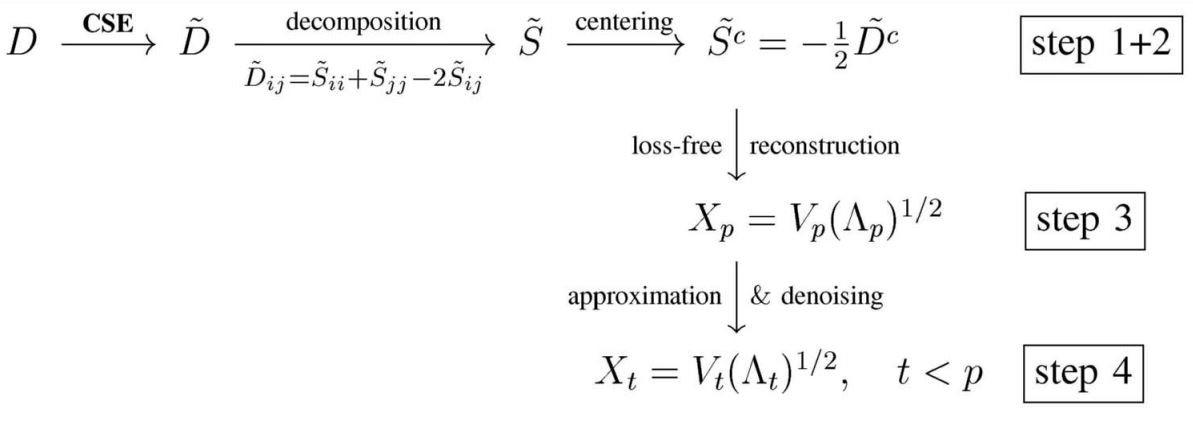
\includegraphics[width=0.9\linewidth]{pictures/reconstructingCSE.jpg}
\end{center}


\subsubsection*{Predicting Cluster Membership of New Data}

\begin{center}
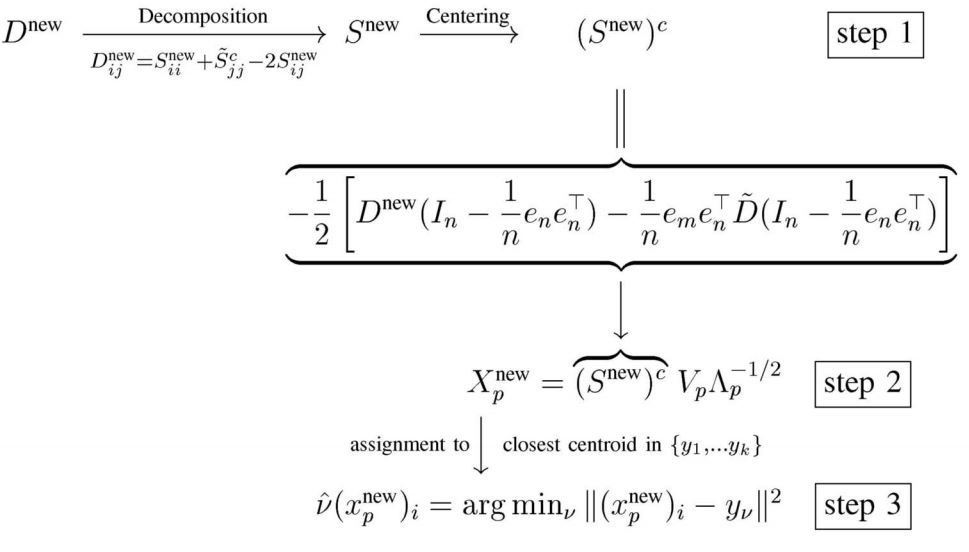
\includegraphics[width=0.9\linewidth]{pictures/predictingClusterCSE.jpg}
\end{center}

\subsection*{Cut}
Partitioning a graph $G(V,E)$ with nodes $V$ and edges $E$ into disjoint sets $A,B$ $\to$ removing edges connecting parts. Degree of dissimilarity is computed as total weight of removed edges: \\
$cut(A,B) = \sum_{u \in A, v \in B} w(u,v)$ \\
\textit{Minimum cut: } optimal bipartitioning of graph that minimizes cut value. \\
Note: Minimum cut favors cutting small sets of isolated nodes in graph. $\to $ use normalized cut.
\subsection*{Normalized Cut}
$Ncut(A,B) = \frac{cut(A,B)}{assoc(A,V)} + \frac{cut(A,B)}{assoc(B,V)}$ where $assoc(A,V) = \sum_{u \in A, t \in V} w(u,t) $
\textit{Ncut(A,B)} can be seen as the disassociation between two groups. \\
 measure for total
normalized association within groups for a given partition:\\
$Nassoc(A,B) = \frac{assoc(A,A)}{assoc(A,V)} + \frac{assoc(B,B)}{assoc(B,V)}$ where $assoc(A,A) $ are the total weights of edges connecting nodes within A, B respectively. Measures how tightly on average nodes are connected within group. \\
$Ncut(A,B) = 2 - Nassoc(A,B)$ \\
\subsection*{Computing Optimal Partition}

\subsection*{Grouping algorithm}
\shadowbox{
\parbox{0.95\linewidth}{
\begin{minipage}{0.75\linewidth}
\begin{enumerate}
\item Given image or image sequence, set up weighted graph $\mathbf{G} = (\mathbf{V},\mathbf{E})$, set weight on edge connecting two nodes to measure of similarity
\item Solve $(\mathbf{D} - \mathbf{W})\mathbf{x}=\lambda \mathbf{D} \mathbf{x}$ for eigenvectors with smallest eigenvalues.
\item use eigenvector with second smallest eigenvalue to bipartition graph by finding splitting point s.t. $Ncut$ is minimized.
\item Decide if current partition should be subdivided by checking stability of cut, make sure $Ncut$ is below prespecified value.
\item recursively repartition if necessary.

\end{enumerate}
\end{minipage}
}
}

\subsubsection*{Computational complexity}
\begin{itemize}
	\item Solving eigenvalue problem for all eigenvectors takes $\mathcal{O}(n^3)$ operations
	\item Graphs often only locally connected, only top few eigenvectors needed, precision requirements low $\to$ $\mathcal{O}(nm) + \mathcal{O}(m M(n))$ where $M(n)$ is the cost of matrix-vector computation $\mathbf{Ax}$ ($A= \mathbf{D}^{1/2}(\mathbf{D} - \mathbf{W})\mathbf{D}^{1/2}$).
\end{itemize}
\section*{Mean Field Approximation}
\subsection*{Mean Field Theory}
Approximate Gibbs distribution by neglecting correlations between stochastic variables $\to$ determine "`most similar"' factorized distribution.
Only consider factorized distributions: 
$q(\mathbf{Z}) = \prod_{i=1}^{M} q_i(\mathbf{Z}_i)$ \\
$\to$ no correlations between assignments of different objects.
Then minimize the Kullback-Leibler divergence to obtain best factorial approximation. \\
Mean field $h_{u \alpha}$ is the expected cost $\mathcal{R}(c)$ that object $u$ assigned to cluster $\alpha$ 

\textit{Mean field upper bound: }
$F(\beta) \leq F_0(\beta) + \langle E \rangle_0 - \langle E_0 \rangle_0 = KL(p_0||p)/\beta + F(\beta) = \sum_{\sigma}p_0(\sigma)E(\sigma) + \frac{1}{\beta} \sum_{\sigma} p_0(\sigma)log_{p_0}(\sigma)$


\subsubsection*{Determine mean field}
\begin{enumerate}
	\item split cost function $\mathcal{R}$ into terms that contain the object $u$ and other terms. Term has a form like $\mathcal{R}(c) = f(u) + \mathcal{R}(c|u)$
	\item take the expected value $\mathbb{E}_{\mathbf{Q}_{u \ to \alpha}}$
\end{enumerate}
\textbf{Pseudocode:}
\begin{center}
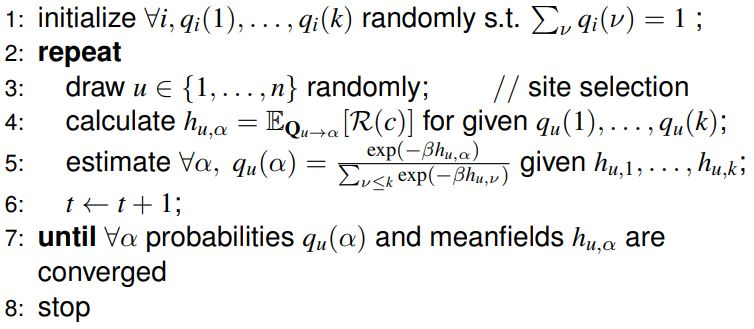
\includegraphics[width=0.8\linewidth]{pictures/meanfields_pseudocode.jpg}
\end{center}
\section*{Approximation set coding}
\textit{Find robust, informative pattern (hypothesis $c\in \mathcal{C}$ hypothesis space) in data }
\subsection*{Approximation sets}
data space $\mathcal{X}$, cost function $\mathcal{R}(c)$, hypothesis $c\in \mathcal{C}$ \\
solution $c^{\bot}(X) = \text{argmin}_{c \in \mathcal{C}} \mathcal{R}(c)$ is random since $X$ is random. \\
$\to$ if second set $X'$ is used $\to c^{\bot}(X) \neq c^{\bot}(X') \, \to$ do not commit to a single answer, use set where each hypothesis $c$ has weight. \\
\subsubsection*{Weights}
weights $w$rank different hypothesis according to how well they solve problem: \\
$\forall c, c' \in \mathcal{C} \, \mathcal{R}(c,X) \leq \mathcal{R}(c,X') \Leftrightarrow w_{\beta}(c,X) \geq w_{\beta}(c,X')$ \\
where approximation precision $\beta$ controls resolution of solutions. \\
$\to$ set of hypothesis that approximately solve the problem: \\$C_{\beta}(X)= \{c \in \mathcal{C} : \, \mathcal{R} (c,X) - \mathcal{R}(c^{\bot}(X),X) \leq 1/\beta \}$ \\
i.e. lead to solutions that are $1/\beta$ close to minimum. \\
assume every $c \in \mathcal{C}_{\beta}$ equally good $\to$ posterior $P_{\beta}(c|X) = \text{unif}(C_{\beta}(X))$ \\
$\beta \to 0$: every hypothesis good solution $\to$ not informative. \\
$\beta \to \infty$: each set has only one element $\to$ not robust. \\
$ \Rightarrow \, \beta$ controls tradeoff between informativeness and robustness/how much posterior distributions agree for different values of $\beta$.

\subsection*{Communication scenario}
\textit{partition hypothesis space $\mathcal{C}$ with distinguishable approximation sets and use them as symbols for communication}
\subsubsection*{Codebook generation}
\textit{Problem:} usually only one set of observations available. $\to$ use set of transformation $\mathbb{T}$: \\
$\forall t \in \mathbb{T}, \forall c \in \mathcal{C}, \forall{\beta} \in \mathbb{R}_{+} w_{\beta}(t \circ c, t \circ X) = w_{\beta}(c,X)$ \\
\textbf{Codebook construction: Script p.g 43}


\subsubsection*{Communication Protocol}

\vspace{5cm}
\begin{itemize}
	\item chain rule for information
\end{itemize}
\section*{Model Selection}
\textit{Minimum Description Length: } $-log p (x|\theta_k) - log p(\theta_k)$ \\

\textit{Bayesian Information Criterion:} $-2 log (\hat p | \hat \theta_k, \mathcal{M}_k)  + k log n$, where $\mathcal{M}_k$ is one of the possible model classes. \\
\textit{Gap Statistic:} $gap_n(k) := E_n^*[log(W_k)] - log(W_k)$, where $W_k = \sum_{\eta}\frac{1}{2n_{\eta}} \sum_{i,j \in \epsilon_{\eta \eta}} D_{ij}$ and $D_{ij} = ||x_i -x_j||^2$
The optimal k can then be chosen as: $k^* = min[k|gap_n(k) \geq gap_n(k+1) - \sigma_{k+1}]$ \\

\textit{Gap Statistic:}
\begin{enumerate}
    \item Train a predictor $\phi_{Z'}$ on the data $Z' := (X', \alpha(X'))$
    \item Predict labels on $X$ using $\phi_{Z'}$
    \item Compare clustering solutions $(\phi_{Z'}(X_i))_{i \in [n]}$ and $\alpha(X)$ on $X$
\end{enumerate}

Choose classifier that matches chosen clustering model. 

\section*{Coding Exercises}
\subsection*{Deterministic Annealing Clustering}
Deterministic Annealing Clustering is an approach to the unsupervised learning problem of clustering. At its core the algorithm is about minimizing the Lagrangian: $$F = D - TH$$
, where $D$ is a measure of the distortion, the "distance" of the datapoints from their respective cluster centers, $H$ is the Shannon Entropy of the system and $T$ is the temperature. The algorithm is grounded in both information theory and statistical physics. The core idea is that, at an initially high temperature the entropy is maximized. Then as we gradually lower the temperature $T$, the distortion is minimized. 

The *preferred implementation* of the algorithm is as follows:
\begin{enumerate}
    \item Initialize the number of codevectors, the minimal temperature, the initial temperature, the initial number of clusters, the initial cluster center and it's probabiltiy. 
\item For i in [1,K] $$y_i = \frac{\sum_x x p(x)(y_i|x)}{p(y_i)}$$ 
    where $$p(y_i|x) = \frac{p(y_i)e^{(x-y_i)^2/T}}{\sum_{j=1}^Kp(y_i)e^{(x-y_j)^2/T}}$$
    and $$p(y_i) = \sum_xp(x)p(y_i|x)$$
\item If not converged, repeat (2)
\item If $T < T_{min}$, stop
\item Cool down: T = $\alpha$ T, $\alpha$ < 1
\item If $K < K_{max}$ check if any of the clusters has reached critical temperature. If so, add a new codevector $y{K+1} = y_j + \delta, p(y_{K+1} = p(y_j)/2, p(y_j) = p(y_j)/2$, where $j$ is the cluster that has reached critical temperature. Increase K by one. 
\item Repeat from (3)
\end{enumerate}


The *critical temperature* is the temperature for which a given cluster splits into two. Assuming Euclidean distance as our measure of distortion, it can be explcitly computed as $$T_{c,y_i} = 2\lambda_{max}$$, where $\lambda_{max}$ is the largest eigenvalue of $C_{x|y_i}$, which in turn is the Covariance matrix of the posterior distribution of $p(x|y)$
\subsection*{Histogram Clustering}
MAP updates:
$\hat{P}(y|c) = \sum_{x \in \hat{c}}{\frac{n(x)}{\sum_{x' \in c}n(x')}\hat{P}(y|x)} $  (1)

$\hat{c}(x) = argmin_{a}\{-\sum_{y\in Y}{\hat{P}(y|x)log\hat{P}(y|a)}\}$  

For DA clustering (1) becomes:
$\hat{P}(y|c)=\sum_{x \in X}\hat{P}(x|c) \hat{P}(y|x)$
with
$\hat{P}(c) = \sum_{x \in X}\hat{P}(c|x)\hat{P}(x)$

$\hat{P}(x|c) = \frac{\hat{P}(c|x)\hat{P}(x)}{\sum_{x \in X}\hat{P}(c|x)\hat{P}(x)}$

and, with

$\hat{P}(c|x) = \frac{exp(-D_{KL}[\hat{P}(.|x)||\hat{P}(.|a)]/T)}{\sum_{b=1}^{K}exp(-D_{KL}[\hat{P}(.|x)||\hat{P}(.|a)]/T)}$ 

replacing equation (6)

\subsection*{DA for pairwise clustering}
Given a dataset of size $N$ and an $N \times N$ dissimilarity matrix $\mathbf{D} = (\mathcal{D}_{ik})$, the problem of pairwise clustering tries to cluster the data into $K$ clusters, represented by an $N \times K$ assignment matrix $\mathbf{M} = (M_{i\nu}) \in \{0,1\}^{N\times K}$ that minimizes the cost function
$$\mathcal{H}^{pc}(\mathbf{M}) = \frac{1}{2} \sum_{i,k=1}^N \frac{\mathcal{D}_{ik}}{N} \left(\sum_{\nu=1}^K \frac{M_{i\nu} M_{k\nu}}{p_\nu} - 1\right)$$
where $p_\nu = \frac{1}{N} \sum_{i=1}^N M_{i\nu}$ is the weight of cluster $\nu$. Algorithm II approximates the Gibbs distribution given by $\mathcal{H}^{pc}$ with the Gibbs distribution given by the factorial cost function $\mathcal{H}^{0}(\mathbf{M}, \mathcal{E}) = \sum_{i=1}^N \sum_{\nu=1}^K M_{i\nu} \mathcal{E}_{i\nu}$, parameterized by external mean fields $\mathcal{E} = (\mathcal{E}_{i\nu})$. Minimizing the Kullback-Leibler divergence $D^{KL}(\mathbf{P}^{Gb}(\mathcal{H}^0)\|\mathbf{P}^{Gb}(\mathcal{H}^{pc})$, where $\mathbf{P}^{Gb}(\mathcal{H})$ is the Gibbs distribution for the cost function $\mathcal{H}(\mathbf{M})$ gives the optimal $\mathcal{E}$ as 
$$\mathcal{E}^*_{i\nu} = \left\langle \frac{1}{1+\sum_{j \neq i} M_{j\nu}} \left[ \frac{1}{2} \mathcal{D}_{ii} + \sum_{k \neq i} M_{k\nu} \left( \mathcal{D}_{ik} - \frac{1}{2} \frac{\sum_{j \neq i} M_{j\nu} \mathcal{D}_{jk}}{\sum_{j \neq i} M_{j\nu}} \right) \right] \right\rangle,$$
where $\left\langle\cdot\right\rangle$ corresponds to taking expectations with respect to $\mathbf{P}^{Gb}(\mathcal{H}^0(\mathbf{M}))$. In the limit of large N, this optimum can be approximated as
$$\mathcal{E}^*_{i\nu} = \frac{1}{1+\sum_{j \neq i} \left\langle M_{j\nu} \right\rangle} \left[ \frac{1}{2} \mathcal{D}_{ii} + \sum_{k \neq i} \left\langle M_{k\nu} \right\rangle \left( \mathcal{D}_{ik} - \frac{1}{2} \frac{\sum_{j \neq i} \left\langle M_{j\nu} \right\rangle \mathcal{D}_{jk}}{\sum_{j \neq i} \left\langle M_{j\nu} \right\rangle} \right) \right].$$
The expectations $\left\langle M_{j\alpha} \right\rangle$ under the Gibbs distribution $\mathbf{P}^{Gb}(\mathcal{H}^0(\mathbf{M}))$ with temperature $T$ are then given by
$$\left\langle M_{j\alpha} \right\rangle = \frac{\exp(-\mathcal{E}^*_{i\alpha}/T)}{\sum_{\nu=1}^K \exp(-\mathcal{E}^*_{i\nu}/T)}$$
Algorithm II then uses deterministic annealing to approximate the Gibbs distribution for varying temperatures, by starting at high temperature, iteratively applying the two above equations for $\left\langle M_{j\alpha} \right\rangle$ and $\mathcal{E}^*_{i\nu}$ in an EM scheme for fixed $T$, and decreasing $T$ exponentially until the final temperature is reached. 

Algorithm III further constrains the variational distribution to be in the form of a Gibbs distribution for the k-means cost function $$\mathcal{H}^{cc}(\mathbf{M}) = \sum_{i=1}^N \sum_{\nu=1}^K M_{i\nu} \|\mathbf{x}_i-\mathbf{y}_\nu\|^2,$$ where $(\mathbf{x}_i)_{i=1}^N$ are embeddings of the data to be determined, and $(\mathbf{y}_\nu)_{\nu=1}^K$ are centroids calculated from $(\mathbf{x}_i)_{i=1}^N$; in this case the mean fields are constrained to take the form $\mathcal{E}_{i\nu} = \|\mathbf{x}_i - \mathbf{y}_\nu\|^2$. Minimizing the KL-divergence $D^{KL}(\mathbf{P}^{Gb}(\mathcal{H}^{cc})\|\mathbf{P}^{Gb}(\mathcal{H}^{pc}))$ with respect to $(\mathbf{x}_i)_{i=1}^N$ and $(\mathbf{y}_\nu)_{\nu=1}^K$ now gives
$$\mathbf{K}_i \mathbf{x}_i \approx \frac{1}{2} \sum_{\nu=1}^K \left\langle M_{i\nu} \right\rangle \left(\|\mathbf{y}_\nu\|^2 - \mathcal{E}^*_{i\nu}\right)\left(\mathbf{y}_\nu - \left\langle \mathbf{y} \right\rangle_i \right)$$
where $\left\langle \mathbf{y} \right\rangle_i = \sum_{\nu=1}^K \left\langle M_{i\nu} \right\rangle \mathbf{y}_\nu$ is the mean of $\mathbf{y}$ under the conditional distribution $p(\nu|i) = \left\langle M_{i\nu} \right\rangle$ and $\mathbf{K}_i = \left\langle \mathbf{y} \mathbf{y}^\top \right\rangle_i - \left\langle \mathbf{y} \right\rangle_i \left\langle \mathbf{y} \right\rangle_i^\top$ the corresponding covariance matrix, and $\mathcal{E}^*_{i\nu}$ is as calculated in Algorithm II.  Algorithm III again uses deterministic annealing, calculating $\left\langle M_{i\nu} \right\rangle^{(t+1)}$ in the E-step from the mean fields $\mathcal{E}^{(t)}_{i\nu} = \|\mathbf{x}^{(t)}_i - \mathbf{y}^{(t)}_\nu\|^2$, and in the M-step updating $\mathbf{x}^{(t+1)}_i$ and $\mathbf{y}^{(t+1)}_\nu$ iteratively from fixed $\left\langle M_{i\nu} \right\rangle^{(t+1)}$ until the variables converge.

\subsection*{MFA for Image Denoising in Ising Model}

In the image denoising setting, we are looking for an image $\sigma$ to minimize:
    $$E(\sigma) = -\lambda \sum_{i=1}^N h_i\sigma - \sum_{i,j = 1}^N J_{i,j} \sigma_i \sigma_j$$
where $h_i$ is the value of pixel $i$ in the noisy observation.
    
 We thus seek to minimize $KL(p_0 || p) + F(\beta)$, which is equivalent to minimizing the Gibbs free energy $G(p)$, where $F(\beta)$ is the free energy, $p_0$ the proposal distribution and $p$ the true distribution.
 
 It can be shown that:
 $$G(p) = -\lambda \sum_{i=1}^N m_i h_i - \sum_{i=1}^{N-1} \sum_{j=i+1}^N m_i J_{ij} m_j$$ \\ $$+ 1/\beta \sum_{i=1}^N (\frac{1 + m_i}{2}log \frac{1 + m_i}{2} + \frac{1 - m_i}{2}log\frac{1 - m_i}{2})$$

where $m_i$ is the mean field for pixel $i$.
Deriving the stationary equations, we find that $G(p)$ is minimized by:
 
 $$m_k = tanh(\beta(\sum_{i\neq k} J_{ki} m_i + \lambda h_k)), k \in {1,N}$$
 
 Which we can solve by iteratively updating the $m_k$.
 
 \subsection*{Model Validation}
 //Some of this stuff is in lecture notes so we might want to cut it.
 In order to compare the stability of cost functions $R(c, \mathbf{X}) \in \mathcal{R}$ under noise in the data $\mathbf{X} \sim \mathbb{P}(\mathbf{X})$, approximation set coding considers a communication scenario including a sender, a problem generator and a receiver. Each entity is initially given access to a sample $\mathbf{X^{(1)}} \sim \mathbb{P}(\mathbf{X})$ and an optimal solution $c^\bot(\mathbf{X^{(1)}}) \in \arg \max_{c\in\mathcal{C}} R(c, \mathbf{X^{(1)}})$. The sender then chooses a transformation $\tau_s \in \mathbb{T}$, $|\mathbb{T}| = 2^{n\rho}$ which acts on the solution space (by permuting elements of the dataset in the case of clustering) and sends it to the problem generator, which generates another sample $\mathbf{X^{(2)}} \sim \mathbb{P}(\mathbf{X})$ and sends $\tau_s \circ \mathbf{X}^{(2)}$ to the receiver. The receiver then estimates $\tau_s$ by maximizing the posterior agreement between $\mathbb{P}(c|\beta, \mathbf{X}^{(1)}) \propto \exp(-\beta R(c,\mathbf{X}^{(1)}))$ and $\mathbb{P}(c|\beta, \tau \circ \mathbf{X}^{(2)}) \propto \exp(-\beta R(c,\tau \circ \mathbf{X}^{(2)}))$, returning $\hat\tau \in \arg \max_{\tau \sum \mathbb{T}} \sum_{c\in\mathcal{C}} \exp(-\beta(R(c,\mathbf{X}^{(1)} + R(c,\tau \circ \mathbf{X}^{(2)}))$. Here $\beta$ represents the degree to which the data is trusted; the larger the noise in the data, the lower $\beta$ has to be chosen to prevent decoding errors. The decoding error $\mathbb{P}(\hat\tau \neq \tau_s|\tau_s)$ can be shown to vanish asymptotically if the rate of transmission $\rho$ falls below the mutual information $$\mathcal{I}_\beta(\tau_s,\hat\tau) = \frac{1}{n} \log \frac{|\{\tau_s\}|\mathcal{Z}_{12}}{\mathcal{Z}_1 \mathcal{Z}_2},$$
where $\mathcal{Z}_1 = \sum_{c\in\mathcal{C}} \exp(-\beta R(c,\mathbf{X^{(1)}}))$, $\mathcal{Z}_2 = \sum_{c\in\mathcal{C}} \exp(-\beta R(c,\mathbf{X^{(2)}}))$, $\mathcal{Z}_{12} = \sum_{c\in\mathcal{C}} \exp(-\beta (R(c,\mathbf{X^{(1)}})+R(c,\mathbf{X^{(2)}})))$ and $|\{\tau_s\}|$ is the number of possible realizations of $c^\bot(\tau_s \circ \mathbf{X}^{(2)})$. 

The approximation capacity is then defined as the maximum of $\mathcal{I}_\beta$ over all inverse temperatures $\beta$. Then to apply model selection on $\mathcal{R}$, we split a given dataset $\mathbf{X}$ randomly into two datasets $\mathbf{X}^{(1)}$ and $\mathbf{X}^{(2)}$, compute the mutual information $\mathcal{I}_\beta$ for each $R \in \mathcal{R}$, maximize it with respect to $\beta$, and choose the cost function with the largest approximation capacity.

For k-means clustering, we have $R(c, \mathbf{X}; \mathbf{Y}) = \sum_{i=1}^n \epsilon_{i,c(i)}$ where $\epsilon_{ik} = \epsilon_{ik}(\mathbf{X}, \mathbf{Y}) = \|x_i - y_k\|^2$ and $\mathbf{Y}$ are the cluster centroids inferred by maximizing the entropy of $\mathbb{P}(c|\beta, \mathbf{X})$. For $\epsilon^{(i)}_{ik} = \epsilon_{ik}(\mathbf{X}^{(i)}, \mathbf{Y})$ the mutual information is calculated as
$$\mathcal{I}_\beta = \frac{1}{n} \log |\{\tau_s\}| + \frac{1}{n} \sum_{i=1}^n \log \frac{\sum_{k=1}^K e^{-\beta(\epsilon^{(1)}_{ik}+\epsilon^{(2)}_{ik})}}{\sum_{k=1}^K e^{-\beta\epsilon^{(1)}_{ik}} \sum_{k=1}^K e^{-\beta\epsilon^{(2)}_{ik}}}$$
where $|\{\tau_s\}|$ is the number of distinct clusterings on $\mathbf{X}^{(1)}$. 

Then to evaluate the approximation capacity of the k-means cost function, we use deterministic annealing to compute the optimal centroids and costs $R(c, \mathbf{X}^{(i)})$ at different temperatures $T = \beta^{-1}$, allowing for $2K$ possible clusters to enable overfitting, and choose as stopping temperature the one with the highest mutual information, balancing informativeness and robustness.

\section*{Exercise Sheets}
\subsection*{Optimal $\beta$ for Expected Log-Posterior Agreement}

We consider the Gibbs posterior over hypotheses:
$p_{\beta}(c|X) = \frac{1}{Z(\beta, X)}exp(-\beta R(c,X))$.
For two data sets X', X', the posterior agreement is defined as: 
$\hat k_{\beta}(X',X'') = \sum_{c \in \mathcal{C}}p_{\beta}(c|X')p_{\beta}(c|X'')$
We want to find $\beta^*$ for which the posterior agreement is maximal. Finding the right $\beta$ can be seen as a trade off between stability and informativeness of the distribution. 
In a sense, the optimal $\beta$ is supposed to give us the most robust solution.
\end{multicols*}



\end{document}





